\documentclass[a4paper,12pt]{article}
\usepackage[slovene]{babel}
\usepackage[utf8]{inputenc}
\usepackage[T1]{fontenc}
\usepackage{lmodern}
\usepackage{amsmath,amsfonts}
\usepackage{enumitem}
\usepackage{graphicx}
\usepackage{subfigure}
\pagenumbering{roman}

\begin{document}

\newcommand{\N}{\mathbb{N}}
\newcommand{\R}{\mathbb{R}}
\newcommand\sbullet[1][.5]{\mathbin{\vcenter{\hbox{\scalebox{#1}{$\bullet$}}}}}
%\theoremstyle{definition} % tekst napisan pokoncno
\newtheorem{definicija}{Definicija}[section]
\newtheorem{primer}[definicija]{Primer}
\newtheorem{opomba}[definicija]{Opomba}


\title{Diskretne Coonsove ploskve}
\author{Matej Rojec, Vito Rozman}
\date{\today}

\maketitle


\newpage

\tableofcontents
\listoffigures

\newpage

\section{Uvod}

V seminarski nalogi bomo obravnavali površine, ki interpolirajo dane mejne krivulje. 
Te površine imenujemo diskretne Consove ploskve, ki jih dobimo z reševanjem linearnega sistema.


Eden od najstarejših problemov v Računalniško podprtem geometrijskem oblikovanju je problem, 
kjer imamo podane štiri robne krivulje, radi pa bi poiskali ploskev z danimi robnimi krivuljami. 
Torej podane imamo robne krivulje $$x(u,0), x(u,1), x(0,v),  x(1,u)$$, kjer lahko brez škode za 
splošnost predpostavimo da je domena ploskve $x(u,v)$ enotni kvadrat $0 <= u,v <=1$. Znana rešitev 
tega problema je bilinearna mešana Coonsova ploskev, ki je interpolirana z robnimi 
krivuljami, kot: 
$$ FORMULA 1.$$ 

\section{Diskretne Coonsove ploskve}
V bolj modernih uporabah CAD, so mejne krivulje Bezierjeve polinomske krivulje, 
ki jih napenjajo kontrolni poligoni. 
\begin{definicija}
    Naj bodo dane točke $\mathbf{b}_0, \mathbf{b}_1, \dots, \mathbf{b}_n$. Potem je Bezierjeva 
    krivulja podana s polinomsko paramerizacijo $\mathbf{p}: [0,1] -> \R^d$ s predpisom 
    $$\mathbf{p}(t) = \sum_{i=0}^n \mathbf{b}_{i} B_i^n(t),$$
    kjer je $B_i^n(t) = \binom{n}{i} t^i (1-t)^{n-i}$, za $i = 0, 1,\dots,n$. Točkam $\mathbf{b}_i$
    pravimo kontolne točke.
\end{definicija}

\begin{definicija}
    Bézierjevo ploskev $\mathbf{p} : [0,1]^2 \rightarrow \R^3$ iz tenzorskega produkta stopnje 
    $(m, n) \in \N \times \N$ definiramo s parametrizacijo:
    $$\mathbf{p}(u,v) := \sum_{i=0}^m \sum_{j=0}^n \mathbf{b}_{i,j} B_i^m(u)B_j^n(v),$$
    kjer sta $(u,v) \in [0,1]^2$ ter $(\frac{i}{m}, \frac{j}{n})$
    domenske točke, ki ustrezajo kontrolni točki $\mathbf{b}_{i,j}$.
\end{definicija}


V tem primeru imamo podane kontrolne točke $b_{i,j}$ opremljene z 
parametroma $(u,v)$ predstavljen s shemo: 
\begin{align*}
    &\mathbf{b}_{0,0} &\mathbf{b}_{1,0} & &\ldots & &\mathbf{b}_{m-1,0} & &\mathbf{b}_{m,0} \\
    &\mathbf{b}_{0,1}  &  & &  & &  & &\mathbf{b}_{m,1} \\
    &\vdots  &  &  & &  & & &\vdots\\
    &\mathbf{b}_{0,n-1}  &  &  & &  & &  &\mathbf{b}_{m,n-1} \\ 
    &\mathbf{b}_{0,n} &\mathbf{b}_{1,n} & &\ldots & &\mathbf{b}_{m-1,n} & &\mathbf{b}_{m,n} \\
\end{align*}
Zgornji FORMULA 1 primer lahko sedaj diskritiziramo in robne krivulje zapišemo s štirimi 
Bezierjevimi krivuljami:
\begin{align*}
    &\mathbf{p}(u,0) =\sum_{i=0}^m \mathbf{b}_{i,0} B_i^n(u), \qquad
    \mathbf{p}(u,1) =\sum_{i=0}^m \mathbf{b}_{i,n} B_i^n(u),  \\
    &\mathbf{p}(0,v) =\sum_{j=0}^n \mathbf{b}_{0,j} B_j^n(v), \qquad
    \mathbf{p}(1,v) =\sum_{j=0}^n \mathbf{b}_{m,j} B_j^n(v),  \\
 \end{align*}
Tako se notranje toče izražajo z na sledeč način: 
$$FORMULA,$$
kjer $0 < i < m$ in $0< j <n$. Izkaže se, da je kontrolni poligon ploskve, 
ki jo omejujejo robne krivulje enak kontrolnemu poligonu, ki ga dobimo z opisano metodo. 
»Morda zanimivo: za določene oblike rabimo definirati samo robne krivulje«.

\begin{figure}[ht!]
   \centering
   \subfigure[Primer robnih točk]{
   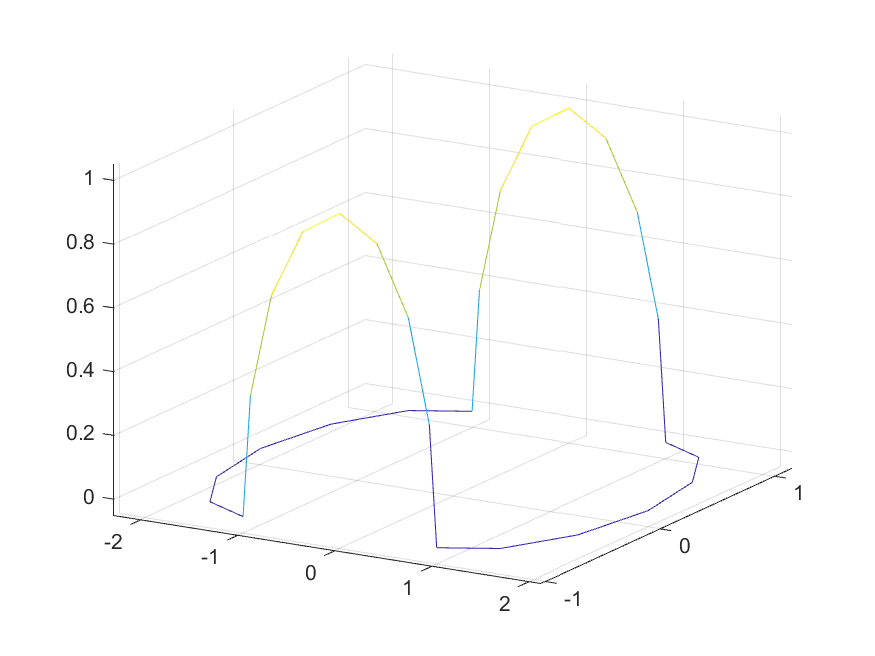
\includegraphics[width=0.45\textwidth]{ogrodje.png}
   }
   \subfigure[Primer ogrodja]{
   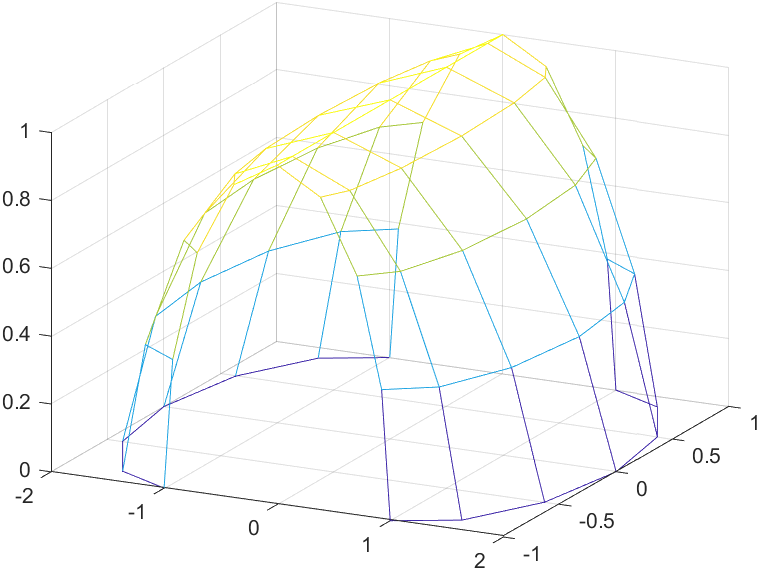
\includegraphics[width=0.45\textwidth]{dodatne_kont_t.png}
   }
   
   \subfigure[Coonsova ploskv na ogrodju]{
   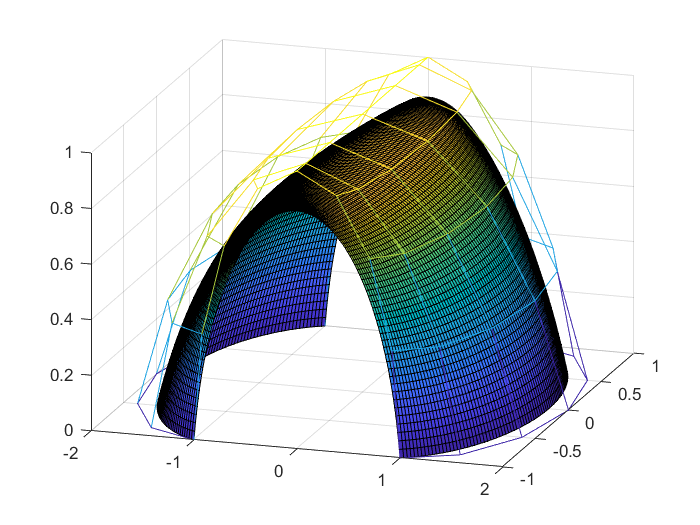
\includegraphics[width=0.5\textwidth]{primer_krivulje.png}
   }   
   \caption{Primer konstrukcije Coonsove ploskve}
\label{fig:whatever}
\end{figure}


\newpage




\section{Lastnosti Coonsovih ploskev}

\subsection{Minimziraje zasuka}
Coonsova ploskve minimzirajo zasuk, definiran kot:
\begin{equation}
   \label{eq:min}
   \int_{[0,1]^2} \left( \frac{\partial^2}{\partial u \partial v}\mathbf{p}(u,v) \right)^2 dS.
\end{equation}
Torej coonsova ploskev doseže minimum izraza.
Posledica tega je, da so Coonsova ploskve lahko v primerih preveč ravne in ne interpolirajo dobro kontrolnih točk.
Taka ploskev prav tako zadošča Euler-Lagrangovi parcialni diferencialni enačbi, torej velja:
\begin{equation}
   \label{eq:pde}
    \frac{\partial^4}{\partial u^2 \partial v^2}\mathbf{p}(u,v) = 0.
\end{equation}

\subsection{Ohranjanje Coonsove ploskve}

Izberimo dve točki $(u_0, v_0)$ ter $(u_1,v_1)$, ki definirajo pravokotnik $P$
v domeni $[0,1]^2$ Coonsove ploskve. 
Robovi pravokotnika $P$ definirajo štiri robne krivulje.
Sedaj tvorimo novo Coonsovo ploskev podano z robnimi krivuljami pravokotnika $P$.
Ta ploskev je enaki Coonsovi ploskvi prvotne krivulje zožane na pravokotnik $P$.

Predpostavimo, da imamo podano ploskev $\mathbf{p}$ iz tenzorskega produkta stopnje $(n,m)$.
Oglejmo si poljubno $3\times 3$ podmrežo podano kot:
\begin{align*}
      &\mathbf{b}_{i-1,j-1} &\mathbf{b}_{i,j-1}& &\mathbf{b}_{i+1,j-1} \\
      &\mathbf{b}_{i-1,j} &\mathbf{b}_{i,j}& &\mathbf{b}_{i+1,j}. \\
      &\mathbf{b}_{i-1,j+1} &\mathbf{b}_{i,j+1}& &\mathbf{b}_{i+1,j+1} \\ 
\end{align*}
V primeru, da poznamo robne točke $3\times 3$ mreže, lahko po zgoraj povedanem
notranjo točko $\mathbf{b}_{i,j}$ izačunamo kot:
\begin{align*}
   \mathbf{b}_{i,j} =&-\frac{1}{4}(\mathbf{b}_{i-1,j-1}+\mathbf{b}_{i+1,j-1}+\mathbf{b}_{i-1,j+1}+\mathbf{b}_{i+1,j+1}) \\
   &+\frac{1}{2}(\mathbf{b}_{i,j-1}+\mathbf{b}_{i-1,j}+\mathbf{b}_{i+1,j}+\mathbf{b}_{i,j+1}).\\
\end{align*}
To lahko zapišemo s pomočjo t.i. maske kot:
\begin{align*}
                                        & &-1  & &2 & &-1 \\
   &\mathbf{b}_{i,j}=\frac{1}{4} \times & 2 & & \sbullet & & 2 .\\
                                        & &-1 & &2 & &-1 \\ 
\end{align*}
Mreža je sestavljena iz $(m+1)\times(n+1)$ kontrolnih točk, od teh ne poznamo 
$(m-1)\times(n-1)$ izmed njih. 
Za vsako izmed $(m-1)\times(n-1)$ imamo natanko eno enačbo, ki je določena z zgoraj opisano masko.
To je seveda zelo časovno zahtevna metoda, da izračunamo kontrolne točke Coonsove ploskve,
ampak nam da nov vpogled, kako bi lahko izračunali kontrolne točke Coonsove ploskve.
Vidimo, da so kontrolne točke Coonsove ploskve poseben primer maske oblike:
\begin{align*}
   & &\alpha  & &\beta & &\alpha \\
&\mathbf{b}_{i,j}= & \beta & & \sbullet & & \alpha,\\
   & &\alpha & &\beta & &\alpha \\ 
\end{align*}
kjer je $(\alpha, \beta) = (-0.25, 0.5)$. To nam, da idejo da bi lahko izbrali različne 
parametra $\alpha$ in $\beta$ sprmenili. Vedno bomo privzeli, da velja $4\alpha + 4\beta = 1$, saj 
tako ohranjamo afinost maske. S perturbiranjem parametrov 
$\alpha$ in $\beta$ dobimo torej nov razred kontrolnih shem. 
Imenujemo jih stalne kontrolne točke. V članku  so raziskovali
vpliv $\alpha$ na optimalno oblike ploskve. Ugotovili so, da za izbrana $m$ in $n$
ni vedno ene optimalne vrednosti za $\alpha$, ki bo dala dobro obliko ploskve.
Namreč optimalna vrednost $\alpha$ je odvisna od oblike robnih krivulj.

\newpage

\begin{thebibliography}{99}
   \bibitem{c1}
   G.~Farin, F.~Hansford, \emph{Discrete Coons patches}, 
   % popravi Morgan \& Claypool Publishers, 2018.
\end{thebibliography}
\end{document}